\documentclass[11pt,a4paper,onecolumn,oneside,notitlepage]{article}
\usepackage[utf8]{inputenc}
\usepackage[english]{babel}
\usepackage{amsmath}
\usepackage{amsfonts}
\usepackage{amssymb}
\usepackage{graphicx}
\usepackage[left=2cm,right=2cm,top=2cm,bottom=2cm]{geometry}

\usepackage[backend=biber, %% Hilfsprogramm "biber" (statt "biblatex" oder "bibtex")
style=authoryear, %% Zitierstil (siehe Dokumentation)
natbib=true, %% Bereitstellen von natbib-kompatiblen Zitierkommandos
hyperref=true, %% hyperref-Paket verwenden, um Links zu erstellen
]{biblatex}
\addbibresource{paper.bib}

\author{Mokrane Yahiatene\\
	\begin{small}
		Deep Learning for Natural Language Processing -- SS21 -- Philipp Cimiano and Philipp Heinisch
	\end{small}
}
\title{SemEval-2020 Task 7: Assessing Humor in Edited
	News Headlines - Subtask 2 (Funnier)}
\begin{document}
	\maketitle
	
	\section{Introduction}
		Humor is a communicative ability resulting in laughter and joy for humans. Assessing text based humor has peaked the interest of many researchers and has been a very challenging task in the Natural Language Processing field.
		The difficulties in assesing funniness lie in the subjective nature of humor. Humans have different tastes in humor and dependends of a lot of factors  f.e.: language,regionality, social status etc.
		Basically a lot of demographic aspects play an important part in finding soemthing humorous.
		If we manage to get good results in generating, detecting and grading humor it would be a huge progress in this scientific field. There would be also quite a few business application for humor assesing (f.e. humor text generating).
		SemEval-2020 Task 7 is a humor-grading task consisting of two subtask(subtask 1, subtask 2) with data from news headlines. These headlines got changed by replacing a single word/entity(micro changes) to make them funnier and afterwards being graded from scores between 0 and 3 , where 0 is the 'least funny' and 3 the 'most funny'.
		The first subtask consists of the originial headline and an edited headline where one must predict the funniness of the edited headline.
		The second subtask comprises of a classification task where one must predict the funnier headline when given two edited headlines(originial1 ,edited1,originial2,edited2).
		This work tries to solve the second subtask with the help of a pretrained transformer model(BERT) .
		
		
	\section{Related work}
		In this section we mainly look at the work \textbf{LRG at SemEval-2020 Task 7: Assessing the Ability of BERT and
		Derivative Models to Perform Short-Edits based Humor Grading} by Siddhant Mahurkar and Rjaswa Patil. 
		They test the ability of BERT and its derivatives (RoBERTa, DistilBERT and ALBERT) in humor grading and classification tasks(subtask 1 and subtask 2) on the Humicroedit and the FunLines dataset.
		Their way of solving both tasks is to create a  BERT model and use the originial weights and  pre trained BERT model weights  fine tuned  with a masked language model layer on top.They compare both weigths results.After that they put a regression layer on top to solve sub task 1. After that they use their model from sub task 1 to solve sub task 2 with zero shot inference. 
		To be precise they followed a masked language modeling approach on the entire dataset only using the edited texts as input while masking all the words in the text for prediction. They chose a maximum sequence length of 256 tokens for masked word prediction. They also experiment with the original BERT Model weights to initiliaze sub task 1 model weights and compare the results.
		Noteworthy is the fact that for sub  task 1 they fed the model the orignial headline and the edited text and for subtask 2 they concatenated the originial headline 1 with the edited headline 1 and concatenated the originial headline 2 with the edited headline 2 and fed the model 2 sentences.
		The reason for that is that the context between the originial end edited headline was deemed important.

	%%    As we can see in figure 2  the differences between the masked and the non masked approach are marginal.

	In this section I use a different approach: similiar to above mentioned approach I concatenated originial headlines with edited headlines but instead of generating 2 sentences I concatenate them again to one sentence in following manner: originial1 + edited1 + originial2 + edited2.
	This new sentence is fed as input into my model which is shown in figure 3.
	My model differs from the usual approach seen in the competition(regression task for task 1 and task 2), instead I'm trying a multi class classification approach with 3 classes. Namely 0,1,2 with the meaning 0: both edited headlines are equally funny, 1 first headline is funnier than second and 2 second headline is funnier than first.
	On top of the vanilla BERT layer I put a Dropout layer and after that an output layer according to my 3 classes with a softmax activation function to get the probabilites for my outputs. 
	I also chose a sequence length of 256 and a batch size of 8 for all my data sets (train,dev,test).
	
	    \begin{figure}
		\begin{center}
			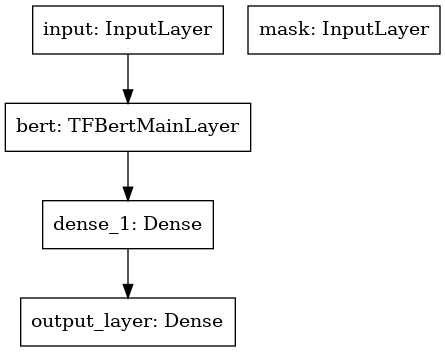
\includegraphics[width=1.0\linewidth]{model.png}
		\end{center}
		
		\caption{Model Architecture}\label{fig3}
	\end{figure}	
		
	\section{Evaluation}
     . See Table \ref{tab1}.
		
		\begin{table}
			\begin{center}
				\begin{tabular}{|c|c|}
					\hline
					\textbf{Model} &  \textbf{Accuracy}\\
					\hline
					\hline
					XXX & 0.6\\
					\hline
					XXX & \textbf{0.8}\\
					\hline
				\end{tabular}
			\end{center}
			
			\caption{Results}\label{tab1}
		\end{table}				
		

	\section{Conclusion}
	In this work we tested the ability of the pretrained BERT Model for state of the art NLP tasks to be precise assesing humor in edited headlines. With little effort one can achieve relatively good results on a custom fine tuned model. Future work could include experimenting with different pretrained models, trying new language model techiques or different approaches in customizing the input. 
	
	\printbibliography
\end{document}